%% BioMed_Central_Tex_Template_v1.06
%%                                      %
%  bmc_article.tex            ver: 1.06 %
%                                       %

%%IMPORTANT: do not delete the first line of this template
%%It must be present to enable the BMC Submission system to
%%recognise this template!!

%%%%%%%%%%%%%%%%%%%%%%%%%%%%%%%%%%%%%%%%%
%%                                     %%
%%  LaTeX template for BioMed Central  %%
%%     journal article submissions     %%
%%                                     %%
%%          <8 June 2012>              %%
%%                                     %%
%%                                     %%
%%%%%%%%%%%%%%%%%%%%%%%%%%%%%%%%%%%%%%%%%


%%%%%%%%%%%%%%%%%%%%%%%%%%%%%%%%%%%%%%%%%%%%%%%%%%%%%%%%%%%%%%%%%%%%%
%%                                                                 %%
%% For instructions on how to fill out this Tex template           %%
%% document please refer to Readme.html and the instructions for   %%
%% authors page on the biomed central website                      %%
%% http://www.biomedcentral.com/info/authors/                      %%
%%                                                                 %%
%% Please do not use \input{...} to include other tex files.       %%
%% Submit your LaTeX manuscript as one .tex document.              %%
%%                                                                 %%
%% All additional figures and files should be attached             %%
%% separately and not embedded in the \TeX\ document itself.       %%
%%                                                                 %%
%% BioMed Central currently use the MikTex distribution of         %%
%% TeX for Windows) of TeX and LaTeX.  This is available from      %%
%% http://www.miktex.org                                           %%
%%                                                                 %%
%%%%%%%%%%%%%%%%%%%%%%%%%%%%%%%%%%%%%%%%%%%%%%%%%%%%%%%%%%%%%%%%%%%%%

%%% additional documentclass options:
%  [doublespacing]
%  [linenumbers]   - put the line numbers on margins

%%% loading packages, author definitions

\documentclass[twocolumn]{bmcart}% uncomment this for twocolumn layout and comment line below
%\documentclass{bmcart}

%%% Load packages
\usepackage{amsthm,amsmath}
\usepackage{siunitx}
\usepackage{mfirstuc}
%\RequirePackage{natbib}
\usepackage[colorinlistoftodos]{todonotes}
\RequirePackage{hyperref}
\usepackage[utf8]{inputenc} %unicode support
%\usepackage[applemac]{inputenc} %applemac support if unicode package fails
%\usepackage[latin1]{inputenc} %UNIX support if unicode package fails
\usepackage[htt]{hyphenat}

\usepackage{array}
\newcolumntype{L}[1]{>{\raggedright\let\newline\\\arraybackslash\hspace{0pt}}p{#1}}

\providecommand{\tightlist}{%
  \setlength{\itemsep}{0pt}\setlength{\parskip}{0pt}}
  
%%%%%%%%%%%%%%%%%%%%%%%%%%%%%%%%%%%%%%%%%%%%%%%%%
%%                                             %%
%%  If you wish to display your graphics for   %%
%%  your own use using includegraphic or       %%
%%  includegraphics, then comment out the      %%
%%  following two lines of code.               %%
%%  NB: These line *must* be included when     %%
%%  submitting to BMC.                         %%
%%  All figure files must be submitted as      %%
%%  separate graphics through the BMC          %%
%%  submission process, not included in the    %%
%%  submitted article.                         %%
%%                                             %%
%%%%%%%%%%%%%%%%%%%%%%%%%%%%%%%%%%%%%%%%%%%%%%%%%


%\def\includegraphic{}
%\def\includegraphics{}

%%% Put your definitions there:
\startlocaldefs
\endlocaldefs


%%% Begin ...
\begin{document}

%%% Start of article front matter
\begin{frontmatter}

\begin{fmbox}
\dochead{Report from 2015 Brainhack at OHBM}

%%%%%%%%%%%%%%%%%%%%%%%%%%%%%%%%%%%%%%%%%%%%%%
%%                                          %%
%% Enter the title of your article here     %%
%%                                          %%
%%%%%%%%%%%%%%%%%%%%%%%%%%%%%%%%%%%%%%%%%%%%%%

\title{Sharing Data in the Cloud}
\vskip2ex
\projectURL{Project URL: \url{https://github.com/DaveOC90/INDI-Organization-Scripts}}

\author[
addressref={aff1, aff2},
corref={aff1},
email={david.oconnor@childmind.org}
]{\inits{DO} \fnm{David} \snm{O'Connor}}
\author[
addressref={aff2},
%
email={daniel.clark@childmind.org}
]{\inits{DJC} \fnm{Daniel J.} \snm{Clark}}
\author[
addressref={aff1, aff2},
%
email={michael.milham@childmind.org}
]{\inits{MPM} \fnm{Michael P.} \snm{Milham}}
\author[
addressref={aff1, aff2},
%
email={ccraddock@nki.rfmh.org}
]{\inits{RCC} \fnm{R. Cameron} \snm{Craddock}}

%%%%%%%%%%%%%%%%%%%%%%%%%%%%%%%%%%%%%%%%%%%%%%
%%                                          %%
%% Enter the authors' addresses here        %%
%%                                          %%
%% Repeat \address commands as much as      %%
%% required.                                %%
%%                                          %%
%%%%%%%%%%%%%%%%%%%%%%%%%%%%%%%%%%%%%%%%%%%%%%

\address[id=aff1]{%
  \orgname{Center for Biomedical Imaging and Neuromodulation, Nathan Kline
Institute for Psychiatric Research},
  \city{Orangeburg},
  \street{140},
  \postcode{10962},
  \postcode{New York},
  \cny{USA}
}
\address[id=aff2]{%
  \orgname{Center for the Developing Brain, Child Mind Institute},
  \city{New York},
  \street{445},
  \postcode{10022},
  \postcode{New York},
  \cny{USA}
}

%%%%%%%%%%%%%%%%%%%%%%%%%%%%%%%%%%%%%%%%%%%%%%
%%                                          %%
%% Enter short notes here                   %%
%%                                          %%
%% Short notes will be after addresses      %%
%% on first page.                           %%
%%                                          %%
%%%%%%%%%%%%%%%%%%%%%%%%%%%%%%%%%%%%%%%%%%%%%%

\begin{artnotes}
\end{artnotes}

%\end{fmbox}% comment this for two column layout

%%%%%%%%%%%%%%%%%%%%%%%%%%%%%%%%%%%%%%%%%%%%%%
%%                                          %%
%% The Abstract begins here                 %%
%%                                          %%
%% Please refer to the Instructions for     %%
%% authors on http://www.biomedcentral.com  %%
%% and include the section headings         %%
%% accordingly for your article type.       %%
%%                                          %%
%%%%%%%%%%%%%%%%%%%%%%%%%%%%%%%%%%%%%%%%%%%%%%

%\begin{abstractbox}

%\begin{abstract} % abstract
	
%Blank Abstract

%\end{abstract}



%%%%%%%%%%%%%%%%%%%%%%%%%%%%%%%%%%%%%%%%%%%%%%
%%                                          %%
%% The keywords begin here                  %%
%%                                          %%
%% Put each keyword in separate \kwd{}.     %%
%%                                          %%
%%%%%%%%%%%%%%%%%%%%%%%%%%%%%%%%%%%%%%%%%%%%%%

%\vskip1ex

%\projectURL{\url{https://github.com/DaveOC90/INDI-Organization-Scripts}}
%\projectURL{https://github.com/DaveOC90/INDI-Organization-Scripts}

% MSC classifications codes, if any
%\begin{keyword}[class=AMS]
%\kwd[Primary ]{}
%\kwd{}
%\kwd[; secondary ]{}
%\end{keyword}

%\end{abstractbox}
%
\end{fmbox}% uncomment this for twcolumn layout

\end{frontmatter}

%{\sffamily\bfseries\fontsize{10}{12}\selectfont Project URL: \url{https://github.com/DaveOC90/INDI-Organization-Scripts}}

%%% Import the body from pandoc formatted text
\section{Introduction}\label{introduction}

Cloud computing resources, such as Amazon Web
Services\footnote{\url{http://aws.amazon.com}} (AWS), provide
pay-as-you-go access to high-performance computer resources and
dependable data storage solutions for performing large scale analyses of
neuroimaging data\cite{Clark2015}. These are particularly attractive for
researchers at small universities and in developing countries who lack
the wherewithal to maintain their own high performance computing
systems. The objective of this project is to upload data from the 1000
Functional Connectomes Project (FCP)\cite{biswal2010} and International
Neuroimaging Datasharing Initiatives (INDI) \cite{mennes2013}
grass-roots data sharing initiatives into a Public S3 Bucket that has
been generously provided by AWS. This will make the data more quickly
accessible for AWS-based analysis of these data, but will also improve
the speed and availability of access to this data for analyses performed
outside of the cloud. To begin with, we focused on the following
collections:

\begin{itemize}
\itemsep1pt\parskip0pt\parsep0pt
\item
  The \emph{Autism Brain Imaging Data Exchange (ABIDE)} consists of
  structural MRI and resting state functional MRI from 1113 individuals
  (164 F, 948 M, 6-64 years old, 539 with autism spectrum disorders, 573
  typical controls) aggregated from 20 different studies
  \cite{dimartino2014}.
\item
  The \emph{ADHD-200} contains structural MRI and resting state
  functional MRI from 973 individuals (352 F, 594 M, 7-21 years old, 362
  with attention deficit hyperactivity disorder (ADHD), 585 typically
  developing controls) collected from 8 sites \cite{Milham2012}.
\item
  The \emph{Consortium for Reliability and Reproducibility (CoRR)}
  consists of 3,357 structural MRI, 5,093 resting state fMRI, 1,302
  diffusion MRI, and 300 cerebral blood flow scans from 1629 subjects
  (673 F, 956 M, 6-84 years old, all typical controls) acquired in a
  variety of test-retest designs at 35 sites \cite{zuo2014}.
\item
  The \emph{Enhanced Nathan Kline Institute - Rockland Sample (ENKI-RS)}
  consists of structural MRI, resting state functional MRI, diffusion
  MRI, cerebral blood flow, and a variety of task functional MRI scans
  and deep phenotyping on over 700 participants from across the lifespan
  and a variety of phenotypes acquired at a single site
  \cite{nooner2012}. The acquisition of this collection is ongoing.
\item
  The \emph{Addiction Connectome Preprocessed Initiative
  (ACPI)}\footnote{\url{http://fcon_1000.projects.nitrc.org/indi/ACPI/html/index.html}}
  consists of 216 structural MRI and 252 functional MRI from 192
  subjects (44 F, 148 M, 18-50 years old) from three datasets generated
  by NIDA investigators.
\end{itemize}

\section{Approach}\label{approach}

Data for the ADHD-200, ABIDE, CoRR, and Rockland Sample data collections
are currently downloadable from
NITRC\footnote{\url{http://fcon_1000.projects.nitrc.org/}} as a series
of large (\textgreater{}2GB) tar files. The process of uploading the
data involved downloading and extracting the data from these tar files,
organizing the individual images, and then uploading the data to S3. We
developed a S3 upload script in python using the Boto AWS software
development kit\footnote{\url{https://aws.amazon.com/sdk-for-python/}}
to facilitate this process. We also developed a download script in
python that provides basic query functionality for selecting the data to
download from a spreadsheet describing the data.

\section{Results}\label{results}

The entirety of the CoRR, ABIDE, ACPI, and ADHD-200 data collections and
ENKIRS data for 427 individuals were uploaded during the OHBM Hackathon
event. The data are available as individual files to make it easily
indexable by database infrastructures such as COINs \cite{landis2016},
LORIS \cite{Das2011}, and others. Additionally, this makes it easy for
the users to download just the data that they want. The data in the
bucket can be browsed and downloaded using a GUI based S3 file transfer
software such as Cyberduck\footnote{\url{http://cyberduck.org}} (see
Fig. 1), or using the Boto python library.

\begin{figure}[h!]
  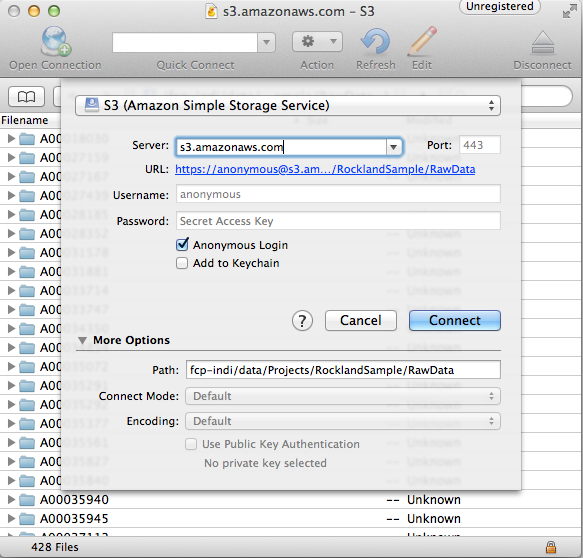
\includegraphics[width=.47\textwidth]{cyberduck_screenshot.png}
  \caption{\label{centfig} Connecting to the data repository.}
\end{figure}

\section{Conclusions}\label{conclusions}

Uploading data shared through the FCP and INDI initiatives improves its
accessibility for cloud-based and local computation. Future efforts for
this project will include uploading the remainder of the FCP and INDI
data and organizing the data in the new brain imaging data structure
(BIDS) format \cite{Gorgolewski2015}.

%%%%%%%%%%%%%%%%%%%%%%%%%%%%%%%%%%%%%%%%%%%%%%
%%                                          %%
%% Backmatter begins here                   %%
%%                                          %%
%%%%%%%%%%%%%%%%%%%%%%%%%%%%%%%%%%%%%%%%%%%%%%

\begin{backmatter}

\section*{Availability of Supporting Data}
More information about this project can be found at: \url{https://github.com/DaveOC90/INDI-Organization-Scripts}. Further data and files supporting this project are hosted in the \emph{GigaScience} repository REFXXX.

\section*{Competing interests}
None

\section*{Author's contributions}
DO performed quality control, and uploaded the data. DJC wrote code to
interact with AWS, preprocessed and uploaded data. MPM and RCC lead the
data collection and sharing projects. All of the authors contributed to
writing the project report.

\section*{Acknowledgements}
The authors would like to thank the organizers and attendees of the OHBM
Brainhack in Hawaii. This project was made possible by the S3 public
bucket generously provided by Amazon Web Services.

  
  
%%%%%%%%%%%%%%%%%%%%%%%%%%%%%%%%%%%%%%%%%%%%%%%%%%%%%%%%%%%%%
%%                  The Bibliography                       %%
%%                                                         %%
%%  Bmc_mathpys.bst  will be used to                       %%
%%  create a .BBL file for submission.                     %%
%%  After submission of the .TEX file,                     %%
%%  you will be prompted to submit your .BBL file.         %%
%%                                                         %%
%%                                                         %%
%%  Note that the displayed Bibliography will not          %%
%%  necessarily be rendered by Latex exactly as specified  %%
%%  in the online Instructions for Authors.                %%
%%                                                         %%
%%%%%%%%%%%%%%%%%%%%%%%%%%%%%%%%%%%%%%%%%%%%%%%%%%%%%%%%%%%%%

% if your bibliography is in bibtex format, use those commands:
\bibliographystyle{bmc-mathphys} % Style BST file
\bibliography{brainhack-report} % Bibliography file (usually '*.bib' )

\end{backmatter}
\end{document}
